\subsection{Экспериментальная апробация}

Экспериментальная апробация направлена на демонстрацию возможностей разработанного предметно-ориентированного языка.

Рассмотрим пример решения некоторой задачи с помощью DSL.
Пусть необходимо получить возраст, имя и пол пользователя и отформатировать ответ в зависимости от его пола.

Первоначально необходимо построить в визуальном конструкторе цепочку блоков для получения имени, возраста и пола пользователя бота.
При получении возраста конвертируем его в числовое значение с помощью специализированного компонента.
Цепочка получения возраста и имени представлена на рисунке~\ref{f:experimentAgeName}.

\begin{figure}[ht]
	\centering
	\vspace{\toppaddingoffigure}
	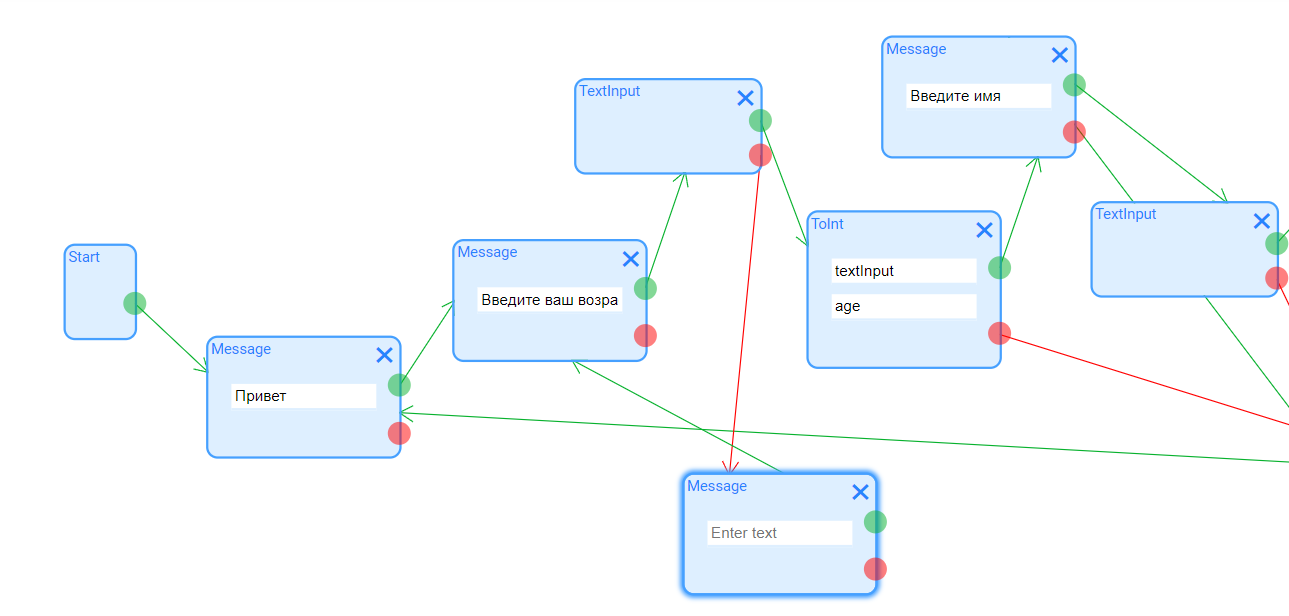
\includegraphics[width=1.0\textwidth]{testing/ageName.png}
	\caption{Цепочка запроса возраста и имени}
	\label{f:experimentAgeName}
\end{figure}

Затем, получим пол пользователя. Для этого отправим пользователю бота сообщение с двумя кнопками,
обозначающими возможные варианты ответа. Если ответ пользователя не будет принадлежать двух возможным вариантам, запрос повторится.
После получения пола пользователя, сохраним его в переменную с помощью компонента <<код>>.
Код возвращает единственное числовое значение в зависимости от выбранного пола: 0 -- был выбран мужской пол, 1 -- женский.
Цепочка получения пола представлена на рисунке~\ref{f:experimentPol}.

\begin{figure}[ht]
	\centering
	\vspace{\toppaddingoffigure}
	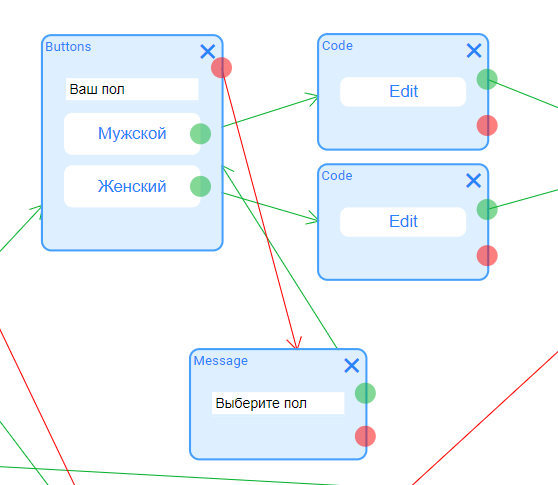
\includegraphics[width=0.8\textwidth]{testing/getPol.png}
	\caption{Цепочка запроса пола пользователя}
	\label{f:experimentPol}
\end{figure}


После того, как были получены все необходимые данные, их можно передать в компонент DSL кода, выполнить над ними некоторые преобразования и вернуть результат.
Пример кода на предметно-ориентированном языке, который формирует ответ в зависимости от пола и прибавляет 5 лет к возрасту пользователя приведен на рисунке~\ref{f:experiment_code}.

\begin{figure}[ht]
	\centering
	\vspace{\toppaddingoffigure}
	\begin{lstlisting}[
        language=Go
    ]

if(code == 1) {
    pol = "Женщина"
} else {
    pol = "Мужчина"
}

m = "Привет, " + textInput + "!
Через 5 лет вам исполнится: " + intToString(age+5) + " лет.

И вы.... " + pol + "! )))";

m
\end{lstlisting}
	\caption{Пример кода на DSL}
	\label{f:experiment_code}
\end{figure}

Цепочка для преобразования данных с помощью компонента кода и отправки завершающего сообщения представлена на рисунке~\ref{f:experimentСodeFinal}.

\begin{figure}[ht]
	\centering
	\vspace{\toppaddingoffigure}
	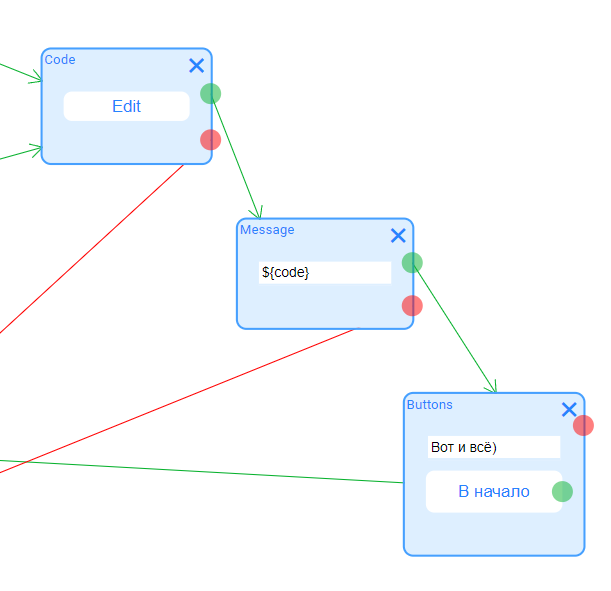
\includegraphics[width=0.7\textwidth]{testing/codeFinal.png}
	\caption{Цепочка с компонентом кода}
	\label{f:experimentСodeFinal}
\end{figure}

Полная сконструированная структура бота представлена на рисунке~\ref{f:experimentFull}.

\clearpage

\begin{figure}[!ht]
	\centering
	\vspace{\toppaddingoffigure}
	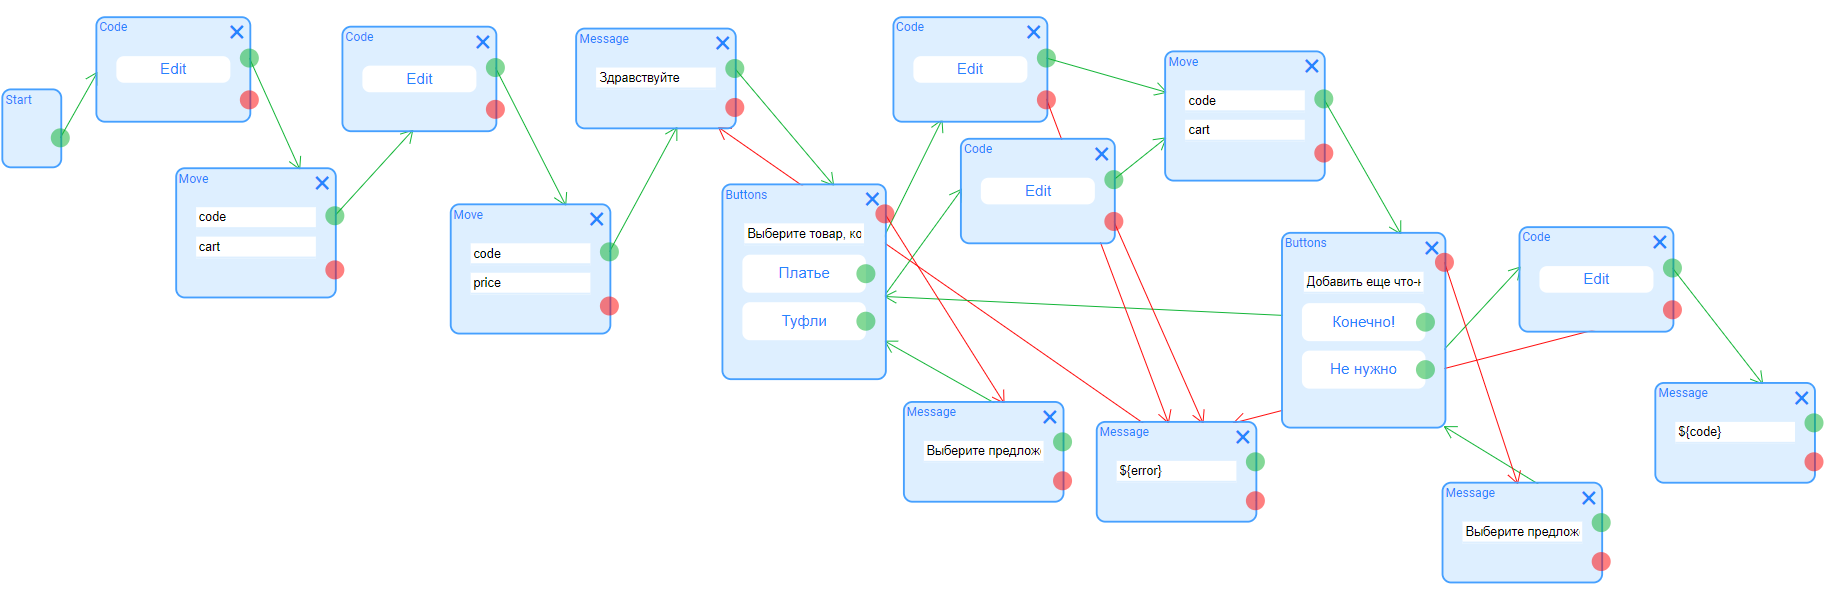
\includegraphics[width=1.0\textwidth]{testing/full.png}
	\caption{Полная компонентная структура бота}
	\label{f:experimentFull}
\end{figure}

Демонстрация работы запущенного Telegram бота представлена на рисунке~\ref{f:experimentDemo}.

\begin{figure}[!ht]
	\centering
	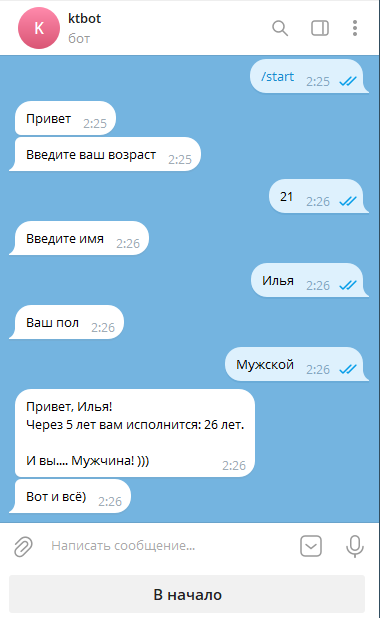
\includegraphics[width=0.45\textwidth]{testing/demo.png}
	\caption{Демонстрация работы бота}
	\label{f:experimentDemo}
\end{figure}

\section*{Вывод}
В данном разделе было проведено тестирование разработанного программного продукта.
На базе встроенной в среду выполнения Go утилиты <<go test>> были реализованы юнит-тесты, охватывающие большинство функций модуля интерпретации.

Также была выполнена экспериментальная апробация, показывающая пример расширения возможностей визуального конструктора Telegram ботов
за счет использования компонента, для запуска кода на разработанном предметно-ориентированном языке.
\clearpage

